\subsection{Momentum Methods}

\begin{frame}{Momentum Methods}
    \frametitle{Accelerating Gradient Descent}
    \begin{itemize}
        \item Momentum methods are designed to accelerate learning, especially in deep, narrow valleys where vanilla gradient descent is slow.
        \item \textbf{The Core Idea:} Keep track of past gradients to build up "velocity" in consistent directions and dampen oscillations in steep directions.
        \item This is analogous to a heavy ball rolling down the error surface; it builds up momentum and is less affected by small bumps and changes in gradient direction.
    \end{itemize}

\end{frame}

\begin{frame}{Momentum Methods}
    \frametitle{Intuition Behind Momentum}
    \begin{figure}
        \centering
        \begin{minipage}{0.5\textwidth}
            \centering
            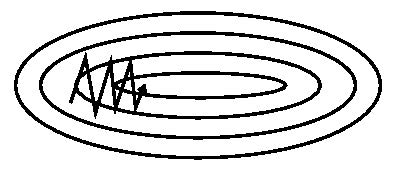
\includegraphics[width=\textwidth]{images/before_momentum.jpeg}
            \captionof{figure}{Plain gradient update}
        \end{minipage}%
            \begin{minipage}{0.5\textwidth}
            \centering
            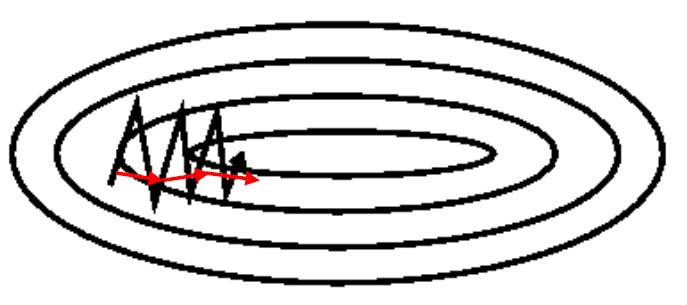
\includegraphics[width=\textwidth]{images/after_momentum.jpg}
            \captionof{figure}{With momentum}
        \end{minipage}
        \caption*{Momentum helps accelerate in consistent directions and dampens oscillations.}
    \end{figure}
\end{frame}

\begin{frame}{Standard Momentum}
    \frametitle{The Momentum Update Rule}
    This method adds a fraction of the previous update vector to the current gradient step.
    \begin{itemize}
        \item A velocity vector, $v$, accumulates an \bhighlight{exponentially decaying moving average} of past gradients.
        \item The update rule is:
            $$ \textcolor{red}{v^{(k)}} = \textcolor{violet}{\beta v^{(k-1)}} + \textcolor{green}{\eta \nabla_w E(W^{(k-1)})} $$
            $$ W^{(k)} = W^{(k-1)} - v^{(k)} $$
        \item $\beta$ is the momentum term, typically set to a value like 0.9 \\ It determines how much of the past velocity is retained.
    \end{itemize}
\end{frame}

\begin{frame}{Nesterov Accelerated Gradient (NAG)}
    \frametitle{A Smarter Momentum}
    Nesterov Accelerated Gradient (NAG) is a slightly different, and often more effective, version of the momentum update.
    \begin{itemize}
        \item \textbf{The Idea:} Instead of calculating the gradient at the current position, NAG "looks ahead" by calculating the gradient at a point where the previous velocity would have taken it.
        \item This allows the optimizer to "correct" its course sooner if the gradient is changing, leading to faster convergence.
        \item The update rule is:
             $$ \textcolor{red}{v^{(k)}} = \textcolor{violet}{\beta v^{(k-1)}} + \textcolor{green}{\eta \nabla_w E(W^{(k-1)} - \beta v^{(k-1)})} $$
             $$ W^{(k)} = W^{(k-1)} - v^{(k)} $$
    \end{itemize}
\end{frame}

\begin{frame}{Visual Comparison: Momentum vs. NAG}
    \frametitle{The "Look-Ahead" Advantage}
    \begin{columns}[T]
        \begin{column}{0.5\textwidth}
            \textbf{Standard Momentum}
            \footnotesize % Using a smaller font for the description
            \begin{enumerate}
                \item Computes gradient at current position.
                \item Adds scaled previous velocity.
            \end{enumerate}
            
            \begin{figure}
                % Placeholder for momentum update diagram from Optimization I.pdf, p. 63
                % Increased width to fill the column
                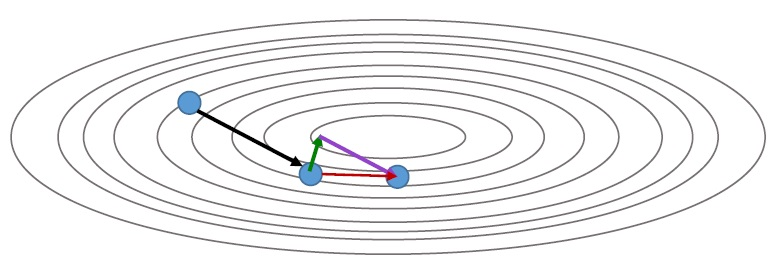
\includegraphics[width=\linewidth]{images/standard_momentum.jpg}
            \end{figure}
        \end{column}
        
        \begin{column}{0.5\textwidth}
            \textbf{NAG}
            \footnotesize % Using a smaller font for the description
            \begin{enumerate}
                \item First, takes a step in direction of previous velocity.
                \item Computes gradient at this "look-ahead" position and makes a correction.
            \end{enumerate}
            
            \begin{figure}
                % Placeholder for NAG update diagram from Optimization I.pdf, p. 70
                % Increased width to fill the column
                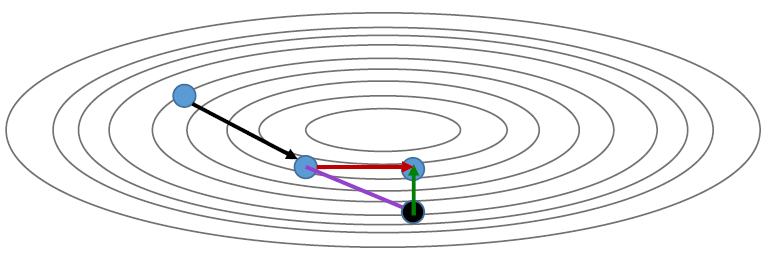
\includegraphics[width=\linewidth]{images/nag.png}
            \end{figure}
        \end{column}
    \end{columns}
    
\end{frame}
